
\section{Introduction to SeismoCloud}

\begin{frame}{Introduction to SeismoCloud}
SeismoCloud is an \textit{early warning system} for earthquakes based on a low
cost sismometers' network.

The goal is to warn residents about an incoming earthquake \textbf{once it
emerged on the epicenter}, within a margin of 5 \circa 20 seconds.

\vspace{1em}
\centering

\includegraphics[keepaspectratio=true,height=40pt]{dipartimentologo}

\includegraphics[keepaspectratio=true,height=40pt]{dipartimento}
\hspace{1em}

\includegraphics[keepaspectratio=true,height=40pt]{ingv}

\end{frame}


\begin{frame}{Introduction to SeismoCloud: map}
\centering
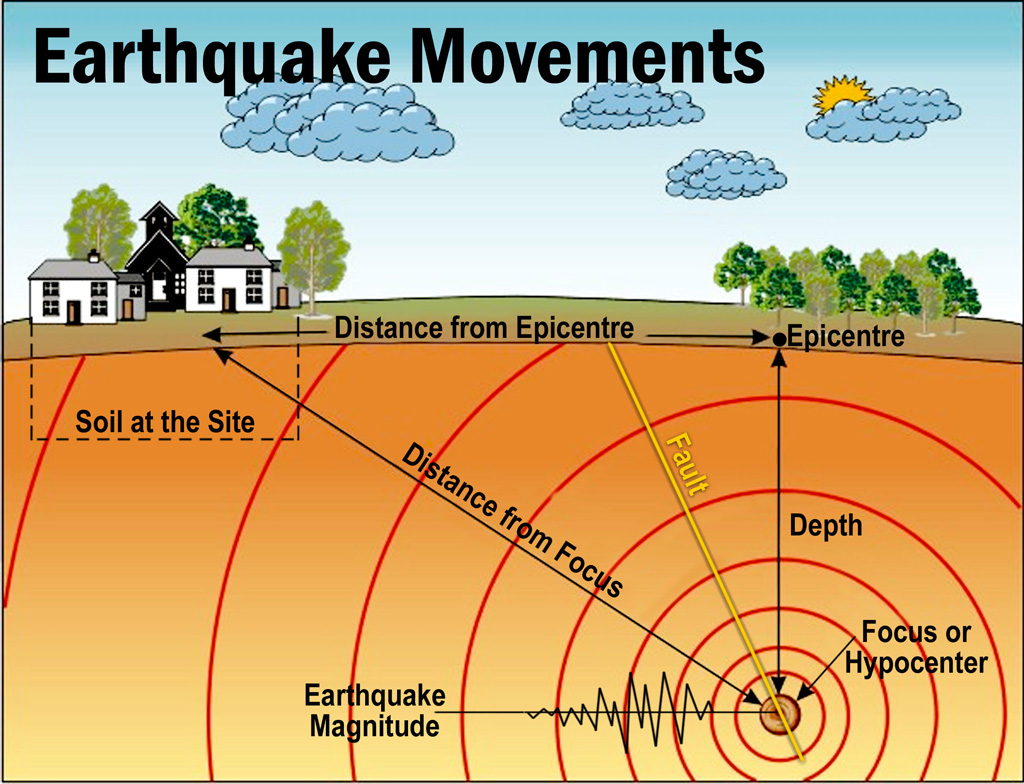
\includegraphics[keepaspectratio=true,width=0.85\textwidth]{earthquake-points}
\end{frame}
